\documentclass[12pt]{article}
\usepackage{ficha}

\begin{document}

\ficha{Transformações de Gráficos de Funções}

\instrucoes{Resolve os exercícios. Considera as transformações: $f(x) + k$, $f(x + k)$, $a\,f(x)$, $f(ax)$, $-f(x)$ e $f(-x)$.}

\secao{Translações}{Descreve a transformação que permite obter o gráfico de $g$ a partir do gráfico de $f$.}
\begin{exercicios}
  \item $g(x) = f(x) + 3$
  \item $g(x) = f(x) - 5$
  \item $g(x) = f(x - 2)$
  \item $g(x) = f(x + 4)$
  \item $g(x) = f(x - 1) + 2$
  \item $g(x) = f(x + 3) - 1$
  \item Se $f(x) = x^2$, escreve a expressão de $g$ obtida por uma translação de vetor $(2, -3)$.
  \item O ponto $(1, 4)$ pertence ao gráfico de $f$. Que ponto pertence ao gráfico de $g(x) = f(x + 2) - 1$?
\end{exercicios}

\secao{Reflexões, Dilatações e Contrações}{Descreve a transformação que permite obter o gráfico de $g$ a partir do de $f$.}
\begin{exercicios}
  \item $g(x) = -f(x)$
  \item $g(x) = f(-x)$
  \item $g(x) = 2f(x)$
  \item $g(x) = \dfrac{1}{3}f(x)$
  \item $g(x) = f(2x)$
  \item $g(x) = f\!\left(\dfrac{x}{2}\right)$
  \item $g(x) = -2f(x) + 1$
  \item O ponto $(4, 6)$ pertence ao gráfico de $f$. Indica um ponto do gráfico de $g(x) = \dfrac{1}{2}f(2x)$.
\end{exercicios}

\secao{Transformações a Partir de um Gráfico}{O gráfico representa a função $f$, de domínio $[-2, 4]$.}

\begin{center}
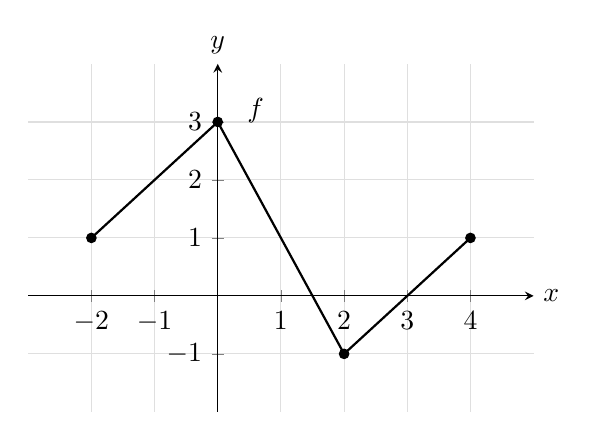
\begin{tikzpicture}
\begin{axis}[axis lines=middle, xmin=-3, xmax=5, ymin=-2, ymax=4, xtick={-2,...,4}, ytick={-1,...,3}, grid=both, grid style={gray!25}, width=8cm, height=6cm, xlabel=$x$, ylabel=$y$, every axis x label/.style={at={(ticklabel* cs:1)},anchor=west}, every axis y label/.style={at={(ticklabel* cs:1)},anchor=south}]
  \addplot[thick, mark=*, mark size=1.5pt] coordinates {(-2,1) (0,3) (2,-1) (4,1)};
  \node at (axis cs:0.6,3.2) {$f$};
\end{axis}
\end{tikzpicture}
\end{center}

\begin{exercicios}
  \item Indica o domínio e o contradomínio de $f$.
  \item Esboça o gráfico de $g(x) = f(x) - 2$ e indica o contradomínio.
  \item Esboça o gráfico de $h(x) = f(x - 1)$ e indica o domínio.
  \item Esboça o gráfico de $i(x) = -f(x)$ e indica o contradomínio.
  \item Esboça o gráfico de $j(x) = f(-x)$ e indica o domínio.
  \item Esboça o gráfico de $k(x) = 2f(x)$ e indica o máximo.
  \item Esboça o gráfico de $m(x) = |f(x)|$.
  \item Indica os zeros de $f$ e os zeros de $p(x) = f(x + 2)$.
\end{exercicios}

\secao{Funções Conhecidas}{Escreve a expressão de $g$ e esboça o gráfico, partindo da função de referência indicada.}
\begin{exercicios}
  \item $f(x) = x^2$; translação de 3 unidades para a direita.
  \item $f(x) = x^2$; reflexão em relação ao eixo $Ox$ seguida de translação vertical de 4 unidades para cima.
  \item $f(x) = |x|$; translação de vetor $(-1, 2)$.
  \item $f(x) = \sqrt{x}$; translação de 2 unidades para a esquerda e 1 para baixo.
  \item $f(x) = \dfrac{1}{x}$; translação de vetor $(3, 1)$. Indica as assíntotas de $g$.
  \item $f(x) = x^3$; dilatação vertical de fator 2 seguida de reflexão em relação a $Oy$.
\end{exercicios}

\secao{Desafios}{Resolve os problemas.}
\begin{exercicios}
  \item Descreve, por ordem, as transformações que levam o gráfico de $y = x^2$ ao gráfico de $y = -2(x - 1)^2 + 3$. Indica o vértice e a concavidade.
  \item A função $f$ tem domínio $[0, 6]$ e contradomínio $[-1, 5]$. Indica o domínio e o contradomínio de $g(x) = 3 - 2f(x + 1)$.
  \item A ordem das transformações importa? Compara $g(x) = 2f(x) + 1$ com $h(x) = 2(f(x) + 1)$ para $f(x) = x^2$.
  \item O gráfico de $g(x) = a(x - b)^2 + c$ tem vértice $(2, -1)$ e passa no ponto $(0, 7)$. Determina $a$, $b$ e $c$.
\end{exercicios}

\end{document}
